\subsection{Konfiguration und Inbetriebnahme}
Um einen Honeypot mit Honeyd zu erstellen muss eine Konfiguration erstellt werden. Als ersten Versuch wurde versucht ein Suse 7.0 Rechner zu simulieren. Dieser blockiert zunächst alle Ports bis auf Port 21 (FTP) und Port 23 (Telnet). ICMP Anfragen werden ebenfalls beantwortet. Die restlichen Ports werden blockiert. Diese eher weniger reale Konfiguration wurde zunächst als Test verwendet. Da die meisten Angriffe auf Honeypots automatisiert ablaufen, dauerte es nicht lange bis die ersten Angriffsversuche auf diesen aufgezeichnet wurden.\\

\begin{figure}[ht]
    \centering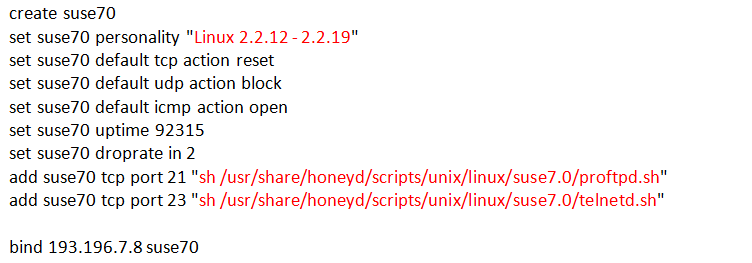
\includegraphics[scale=0.7]{Bilder/Suse70.png}
  \caption{Erst Testkonfiguration mit Honeyd}
  \label{suse70}
\end{figure}

Durch ein Problem mit der veralteten Version von Honeyd hörte der Deamon meist nach einiger Zeit mit dem Aufzeichnen der Angriffe auf. Da es zu diesem Problem keinerlei Fehlermeldung gab und das Projekt nicht mehr weiter verfolgt wurde gelang es nicht diesen Fehler zu beheben. Durch mehrere Neustarts des NEtzwerkinterfaces und der Deamons konnten jedoch einige Angriffe aufgezeichnet werden. 

Die zweite Testkonfiguration ist ein Windows XP Konfiguration. Diese besitzt nur leicht andere Konfigurationseinstellungen als das zuvor verwendete Suse 7.0 Skript. Da das Problem mit dem Abbruch der Aufnahmen weiterhin bestand, machte es keinen Unterschied welche Konfiguration verwendet wurde, die Angriffe waren meist identisch.\\

\begin{figure}[ht]
    \centering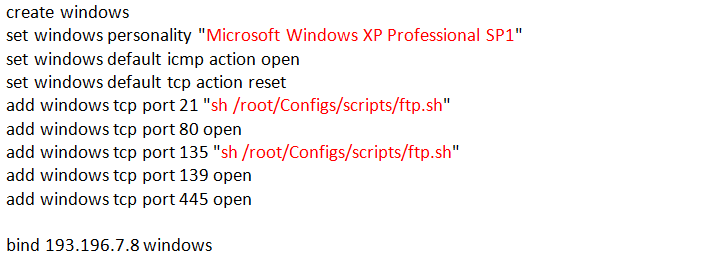
\includegraphics[scale=0.7]{Bilder/WinXP.png}
  \caption{Zweite Testkonfiguration mit Honeyd}
  \label{winXP}
\end{figure}

\noindent Trotz das nur wenige Daten aufgezeichnet werden konnten wurde der Honeypot jedes mal kurz nach Produktivstellung angegriffen. Was für Angriffe dies waren wird im folgendem Kapitel genauer betrachtet.